%!TEX root = ../thesis.tex
%*******************************************************************************
%*********************************** Sixth Chapter *****************************
%*******************************************************************************

\chapter{Simulation study for  CPACE model \label{cha:application}}  %Title of the Sixth Chapter

\ifpdf
    \graphicspath{{Chapter6/Figs/Raster/}{Chapter6/Figs/PDF/}{Chapter6/Figs/}}
\else
    \graphicspath{{Chapter6/Figs/Vector/}{Chapter6/Figs/}}
\fi
The CPACE model as described in Chapter~\ref{cha:cpace} is designed to allow for functional data which are observed dependently.
Most often this may be a spatial dependence between neighbouring trajectories although the framework discussed isn't reliant on this.
We have shown theoretically how we would reconstruct unobserved trajectories using our estimators. 
However, we are yet to highlight in practice the ability of such estimators and their reconstruction ability.
In the following chapter we present a series of simulated results designed to test the estimator capabilities, namely the ability to recover model hyper parameters and its reconstruction ability for unobserved locations.
We contrast the CPACE models results against the traditional FPCA PACE model which doesn't utilise the spatial information of the functional data.

\section{Simulation Study \label{sec:sim_study}}
In the following section we present a simulation study based on the simulation study of \cite{yao_functional_2005}.
This simulation study was designed in \cite{yao_functional_2005} to showcase the implementation of sparse functional principal components analysis which are observed independently.
We will take this study as a base and then develop their generating procedure to allow for spatial dependency between functional observations.
We refer, in the following, to spatial dependency between functional observations because our main application of the CPACE model is the EO data, which naturally has spatial dependency.
However, this simulation study, and indeed the CPACE model can naturally be applied with different dependency between functional observations.

The simulation study consists of four scenarios; namely A, B, C, and D.
In each scenario the functional data are generated from the same mean and principal components.
We vary the spatial dependence between each scenario to show how the CPACE model with different spatial kernels can accommodate differing spatial structures.
We detail the exact specification for each scenario in its respective subsection.
First we describe the common underlying data generating process for the functional data.

\subsection{Data Generating Process \label{ssec:dgp_sim}}
We propose the simulations to be generated over temporal domain $\mathcal{T} \in \left[0, 10\right] \subset \mathbb{R}$.
The processes have mean, $\mu\left(t\right) = t + \sin\left(t\right)$, and generated as in Equation \eqref{eqn:fpca_cpace} with $K=2$.
The eigenfunctions are given by: 
\begin{eqnarray}
	\phi_1\left(t\right) &=& -\frac{1}{\sqrt{5}}\cos\left(\frac{\pi t}{10}\right) \nonumber \\ 
	\phi_2\left(t\right) &=& -\frac{1}{\sqrt{5}}\sin\left(\frac{\pi t}{10}\right) \nonumber \\
\end{eqnarray}

Figure~\ref{fig:sim_mean} displays the mean function we use for the simulation, and Figure~\ref{fig:sim_eig} highlights the variation from the mean function that each eigenfunction contributes.
As can be seen, the mean function used for the simulation has a clear upward trend and a periodic component.
The first eigenfunction represent periodic variation at the start and end of the temporal domain, with the second eigenfunction giving variation in the middle of the temporal domain.

\begin{figure}
	\centering
	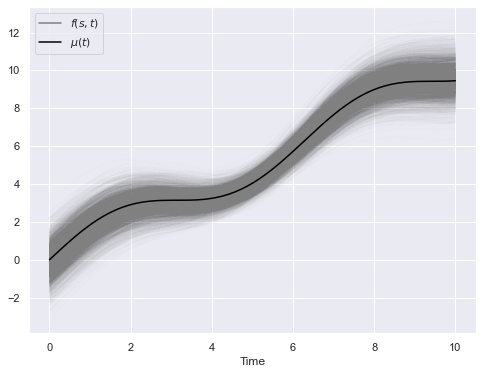
\includegraphics[width=\textwidth]{mean_sim}
	\caption{The mean function chosen for the simulation study over the temporal domain. We have illustrated example functional data simulated using this mean function in grey.}
	\label{fig:sim_mean}
\end{figure}

\begin{figure}
	\centering
	\begin{subfigure}[b]{0.45\textwidth}
		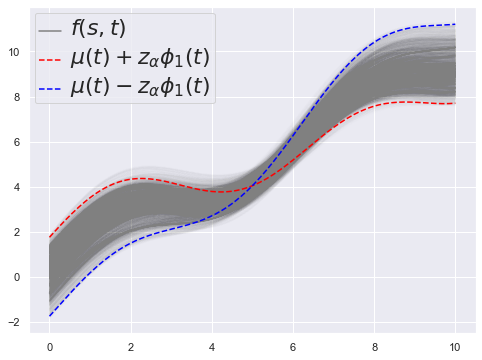
\includegraphics[width=\textwidth]{sim_eig_1}
		\caption{Variation from the mean function caused by the first eigenfunction.}
		\label{fig:sim_eig1}
	\end{subfigure}
	\hfill        
	\begin{subfigure}[b]{0.45\textwidth}
		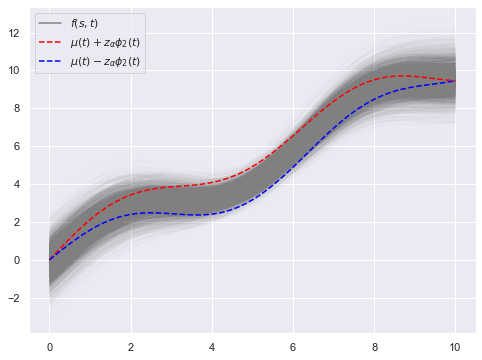
\includegraphics[width=\textwidth]{sim_eig_2}
		\caption{Variation from the mean function caused by the second eigenfunction.}
		\label{fig:sim_eig2}
	\end{subfigure}
	\caption[An example of the variation due to the two eigenfunctions from the mean function. ]{An example of the variation due to the two eigenfunctions from the mean function. The kernel variance chosen for this study is $\lambda_1 = 4$ and $\lambda_2 = 1$ (Discussed in detail below). We illustrate the impact of this variation with a z-score corresponding to $\alpha=0.05$.  That is that there is a $95 \%$ probability that the mean plus the respective eigenfunction lies within the upper and lower bounds. Again we highlight example functional data generated from this setup in grey.}
	\label{fig:sim_eig}
\end{figure}

We propose to simulate observations on the spatial domain of $\mathcal{S} = \left[-5, 5\right] \times \left[-5, 5\right] \subset \mathbb{R}^2$.
We choose this spatial domain without great consideration as we can always rescale our input to this domain.
It so happens that this scale for the domain allows for us to flexibly choose scenarios with varying degrees of spatial dependency.
Each location $\ve{s} \in \mathcal{S}$ can give rise to a functional data generated by the above mean and principal components by Equation \eqref{eqn:fpca_cpace}.
In order to generate such data in practice we discretise the temporal domain to a fine grid by segmenting $\mathcal{T}$ into $128$ equal segments, and use the midpoints for generation of the functional data.
For each functional observation we suppose, as in \citep{yao_functional_2005} and our setup in Chapter \ref{cha:Into}, that we do not observe the full true function $\mathcal{X}\left(\ve{s}, t\right)$ but we sparsely observe a noisy version of it.
For all the simulations we suppose our noise variance is $\sigma^2_\epsilon = 0.25$. 
We set the sparsity of observations to be between $5\%$ and $10\%$ of our full $128$ temporal grid.
This is in line with the simulation study of \citeauthor{yao_functional_2005}.
That is, our number of observation points are chosen uniformly from $\left[6, 7, \cdots, 11, 12\right]$.
The observation points are sampled randomly from the full discretized grid over $\mathcal{T}$.
This is a slight deviation from the simulation study in \citep{yao_functional_2005} but lies closer to reality for EO data which is often observed at regular grid intervals.
Figure~\ref{fig:sim_example} highlights an example of the sparsity and observation error described above.

\begin{figure}
	\centering
	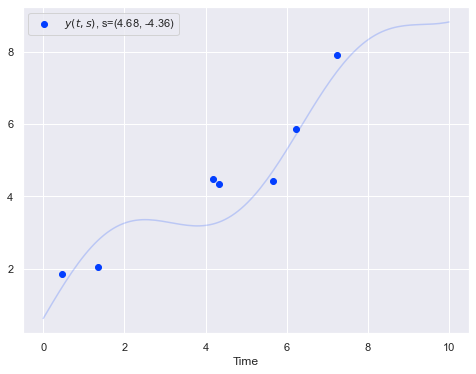
\includegraphics[width=\textwidth]{sim_ex}
	\caption{An example functional data with observation points. This example is taken from Scenario A and highlights the sparsity of observation as well as the impact of the noise variance on observations.}
	\label{fig:sim_example}
\end{figure}

For the spatial domain, $\mathcal{S} \subset \mathbb{R}^2$ we take a similar approach.
Again in practice we discretize this into $64$ equally spaced segments across the first domain, and $48$ equally spaced segments across the second domain.
We take the midpoints as our discretized sampling locations.
This gives in total $64 \times 48$ possible sampling locations for our simulation study.
We take half of our sampling locations as observed data, that is used to estimate the parameters of the CPACE model.
Namely, the spatial kernel hyper-parameters and eigen decomposition parameters.
As we only observe each functional datum sparsely this corresponds to a training dataset of approximately $3.75\%$ of the total discretized points of simulation.

As stated above, to simulate spatially dependent functional data we must simulate a realisation of our spatial covariance process $\xi_i(\ve{s})$ for $i=1,2$. 
The particular form of this process will change in each scenario but we keep the variance of these processes consistent to align closely with the study in \citep{yao_functional_2005}.
That is we set the variance of $\xi_1$ to be $4$ and $\xi_2$ to be $1$, which corresponds to $\lambda_1 = 4$ and $\lambda_2=1$ from Chapter~\ref{cha:cpace}.

Finally, we simulate $50$ replications using the above data generating procedure to produce our scenario dataset.
For each simulation of each scenario we will evaluate various versions of the CPACE model against the standard FPCA model which doesn't take into account the spatial correlation between functional observations.
We discuss the evaluation of our models against these simulated data in the following section. 

\subsection{Evaluation metrics \label{ssec:eval_metrics}}
To evaluate the performance of our model we consider two standard metrics; the mean square error, and the mean absolute error.
These are standard evaluation metrics for a regression based model but for clarity the mean square error and mean absolute error for prediction $\hat{\mathcal{X}}$ against unobserved functional data $\mathcal{X}$ is given by:

\begin{eqnarray}
	MSE = \frac{1}{50} \sum_{i=1}^{50} \int \int \left( \hat{\mathcal{X}}(\ve{s}, t) - \mathcal{X}(\ve{s}, t) \right)^2 d\ve{s} dt \nonumber \\
	MAE = \frac{1}{50} \sum_{i=1}^{50} \int \int \left| \hat{\mathcal{X}}(\ve{s}, t) - \mathcal{X}(\ve{s}, t) \right| d\ve{s} dt \nonumber
\end{eqnarray}
In practice, we evaluate these on the discrete simulation grid and use numerical integration to approximate these metrics.

For our simulation study we have three distinct sets of data to evaluate performance against.
The training data set, which comprises solely of the location and time points for which we observe, noisily, the functional data.
The validation dataset which comprises of the locations of where we observe our noisy data, but including unobserved time points. 
Finally, the test dataset which comprises of completely unseen locations and time points.

Comparing the performance of the CPACE model against the standard FPCA model against each dataset should highlight how well our CPACE model performs under the three separate conditions.
Greater performance on the test dataset is most preferable as it provides insight into functions at unobserved locations.
To place back in the context of EO data, this could be useful to interpolate data where it is not possible to get physical observations.
The validation dataset highlights the ability of the model to recover observations from a possibly malfunctioning data source which leads to partial observations at a particular location.
The training dataset is typically the easiest to achieve good performance on and is most suitable for evaluation of the model's ability to overcome observation error.

In this study we will examine the performance of the CPACE model with four different spatial kernels.
Three of these correspond to stationary kernels, and one is designed to model non-stationary spatial dependence. We detail them below: 

\subsection{Spatial Kernels  \label{ssec:spatial_kern}}
We choose four kernels to examine. The first of which corresponds to the kernel with no spatial dependence, and is chosen to highlight the ability of the CPACE model to recreate the PACE model. 
The next two correspond to common spatial kernels using the Mat\'ern covariance form, one of which is used in the SPACE model, \citep{liu_functional_2017}. These highlight the CPACE model's ability to capture quite simplistic spatial correlation structures.
The final, is a less commonly used kernel which capture non-stationarity in the spatial dependence.
This kernel is chosen to highlight that the CPACE model can effectively be used in cases of highly complex spatial dependence.
As in Chapter~\ref{cha:background} we refer the reader to \cite{cressie_statistics_2011} for a more in depth discussion of various covariance structures in spatial statistics.

\subsubsection{White Kernel \label{sssec:white_kern}}
The White, or Independent kernel, is the simplifying assumption which reverts the CPACE model to the standard PACE model. That is it defines the covariance between $\vesub{s}{i}$ and $\vesub{s}{j}$ as follows:

\begin{equation}
	\xi_k\left(\vesub{s}{i}, \vesub{s}{j}\right) = \lambda_k\delta_{ij}
\end{equation}
where 
\begin{equation*}
\delta_{ij} = \begin{cases}
	1 & \text{if } \vesub{s}{i} = \vesub{s}{j}, \\
	0 & \text{otherwise}
\end{cases} 
\end{equation*}

This kernel places zero correlation between functional data at differing spatial locations, and a variance of $\lambda_k$ for functional observations at the same locations.
Note that this corresponds to the full cross-correlation of $\mathcal{X}\left(\vesub{s}{i}, t \right)$ and  $\mathcal{X}\left(\vesub{s}{j}, t \right)$ under our initial example given by Equation~\ref{eqn:principal_comp_uncorr} in Chapter~\ref{cha:background}.
The added distinction that we are now using  is the use of parameter $\ve{s}$ to indicate spatial location over the domain $\mathcal{S}$ rather than an simple discrete index.
As such the use of this kernel in the CPACE model will result in essentially a differing view of the PACE model under which there is assumed no spatial correlation.

\subsubsection{Mat\'ern One Half Kernel \label{sssec:matern_one}}
The Mat\'ern kernel is a standard in the spatial statistics literature, \cite{cressie_statistics_2011}.
The general form in our setting is given by, \citep{cressie_statistics_2011}:
\begin{equation}
	\xi_k\left(\vesub{s}{i}, \vesub{s}{j}\right) = \lambda_k \frac{2^{1-\nu}}{\Gamma(\nu)}\left(\sqrt{2\nu} \frac{d}{\rho}\right)^\nu K_\nu \left(\sqrt{2\nu} \frac{d}{\rho}\right)
	\label{eqn:gen_mat}
\end{equation}
where $d = \lVert \vesub{s}{i} - \vesub{s}{j} \rVert$, $K_\nu$ is the Modified Bessel function of the second kind, $\Gamma$ is the gamma function, $\rho$ is a length scale parameter, and $\nu$ is a parameter controlling the shape of the covariance.
The Mat\'ern One Half kernel is a specific example of the general form by setting $\nu=0.5$ in Equation~\ref{eqn:gen_mat}. 
When setting this shape parameter it leads to a simple closed form, given below:

\begin{equation}
	\xi_k\left(\vesub{s}{i}, \vesub{s}{j}\right) = \lambda_k \exp \left( -\frac{d}{\rho} \right)
\end{equation}

This kernel is often used due to its simplicity to compute while it maintains good ability to capture stationary covariances.
We use the Euclidean distance for the calculation of $d$ which makes this kernel isotropic.
The length scale parameter, $\rho$, is used to capture the correlation over differing spatial scales.
In the CPACE model we treat $\rho$ as a hyper parameter to estimate.
This estimation procedure is described in Chapter~\ref{cha:cpace} with more implementation details in Chapter~\ref{cha:implementation}.
Figure~\ref{fig:ex_mat_1} shows the covariance on our spatial domain $S$ with length scale, $\rho = 1.5$,  and variance $\lambda_k$ equal to $1$ .

\begin{figure}
	\centering
	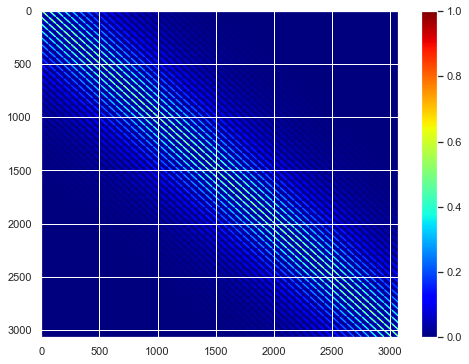
\includegraphics[width=\textwidth]{ex_mat_1}
	\caption[Example Mat\'ern One Half covariance]{The covariance between all points in out spatial domain $\mathcal{S}$ with the Mat\'ern One Half covariance function with $\rho=1.5$ and $\lambda=1$. Each index on the axis corresponds to a point $\ve{s}_i$ in $\mathcal{S}$ in our discretised grid.}
	\label{fig:ex_mat_1}
\end{figure}

The use of this model is akin to the SPACE model, \citep{liu_functional_2017}.
However in the CPACE model the estimation procedure for hyper parameters is different.

\subsubsection{Mat\'ern Three Halves Kernel \label{sssec:matern_three}}
Similar to the Mat\'ern One Half kernel this is another specific example of the general Mat\'ern covariance kernel.
This time we set the shape parameter $\nu$ to $1.5$ in Equation~\ref{eqn:gen_mat}.
This leads to the specific closed form of the covariance kernel given below:

\begin{equation}
	\xi_k \left(\vesub{s}{i}, \vesub{s}{j}\right) = \lambda_k \left(1 + \frac{\sqrt{3}d}{\rho} \right)\exp \left(\frac{- \sqrt{3}d}{\rho} \right)
\end{equation}
where again $d$ is the Euclidean distance between $\vesub{s}{i}$ and $\vesub{s}{j}$ given by $d = \lVert \vesub{s}{i} - \vesub{s}{j} \rVert$. 
Again, this is a stationary kernel, that is the covariance between two points depends only on the spatial distance between points and not their location.
The length scale parameter, $\rho$, is used to capture the correlation over differing spatial scales.
In the CPACE model we treat it as a hyper parameter to estimate.
Figure~\ref{fig:ex_mat_3} shows an example covariance structure over our spatial domain $\mathcal{S}$ for the simulation study with $\rho =1.5$ and $\lambda = 1$.
We note that comparing this to Figure~\ref{fig:ex_mat_1} that the covariance model is naturally smoother that the Mat\'ern One Half kernel and in some sense is designed to model smoother variation over the domain.

\begin{figure}
	\centering
	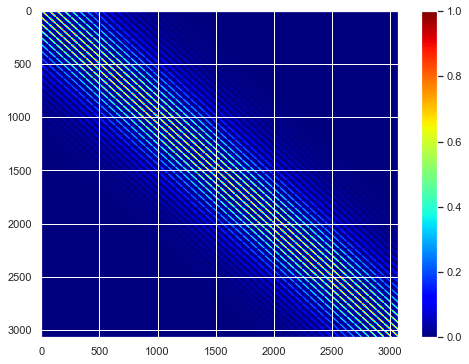
\includegraphics[width=\textwidth]{ex_mat_3}
	\caption]Example Matern Three Halves covariance]{The covariance between all points in out spatial domain $\mathcal{S}$ with the Mat\'ern Three Halves covariance function with $\rho=1.5$ and $\lambda=1$. Each index on the axis corresponds to a point $\ve{s}_i$ in $\mathcal{S}$ in our discretised grid.}
	\label{fig:ex_mat_3}
\end{figure}

Again, the use of this model is akin to the SPACE model, \citep{liu_functional_2017}.
However in the CPACE model the estimation procedure for hyper parameters is different.

\subsubsection{Gibbs Kernel \label{sssec:gibbs}}
All the above kernels are stationary.
Stationary kernels have been well studied due to the relative ease of estimation of kernel hyper parameters.
However, they are often too simplistic as many real world data sets exhibit some form of non-stationarity.
We consider the Gibbs kernel, named after the Gibbs who authored the thesis which first described this kernel, \citep{gibbs_bayesian_1998}, in our simulation study as a non-stationary kernel which can account for more complex spatial dependence.
The form of the kernel is given succinctly by \citeauthor{paciorek_spatial_2006}, \citep{paciorek_spatial_2006}, for one dimensional input. 

\begin{equation}
	\xi_k\left(s_{i}, s_{j}\right) = \lambda_k \sum_{q=1}^{Q} \sqrt{\frac{2l_q(s_i)l_q(s_j)}{l_q(s_i)^2 + l_q(s_j)^2}} \exp \left(-\frac{\left(s_i - s_j\right)^2}{l_q(s_i)^2 + l_q(s_j)^2}\right)
\end{equation}

This can be simply extended to two, as in our simulation case, or more dimensions by having a Gibbs kernel on each dimension of the input and combining by simply multiplying them together.
This remains a valid positive definite kernel as the product of two or more positive definite kernels remains positive definite. 
In this Gibbs kernel we have multiple components, referenced by $Q$ total components.
Each component has its separate length scale model $l_q(s)$ which controls the length scale parameters at each point in the domain.
In principal these length scale models can be arbitrary positive functions, and the Gibbs kernel remains valid.

Figure~\ref{fig:ex_gibbs} gives an example covariance function from the Gibbs kernel.
As can be seen, the covariance structure changes over the domain, highlighting the non-stationarity of the Gibbs model.
This can allow for much more complex spatial structures.
Here we have restricted the kernel to two components, and use as in Scenario D, the lengthscale model given by:
\begin{eqnarray}
	l_1(s) &=& \frac{1}{1 + \exp(-s)} \nonumber \\
	l_2(s) &=& \frac{1}{1 +  \exp(s)} \nonumber \\
\end{eqnarray}
For example, locations in the middle of the domain $\mathcal{S}$, are less correlated to immediate neighbours than the locations on the fringes of the domain.
This has been induced by the choice of the length scale models above.
In our simulation study, we treat these as hyper parameters to be estimated from the observed data.
The way in which we do so will be discussed in greater detail in Section~\ref{sec:sim_D} and in Chapter~\ref{cha:implementation}.

\begin{figure}
	\centering
	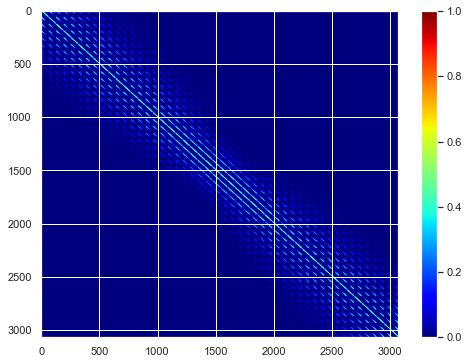
\includegraphics[width=\textwidth]{ex_gibbs}
	\caption{The covariance between all points in out spatial domain $\mathcal{S}$ with the above covariance function. Each index on the axis corresponds to a point $\ve{s}_i$ in $\mathcal{S}$ in our discretised grid.}
	\label{fig:ex_gibbs}
\end{figure}

Now we discuss the specific results of using the various kernels in our simulation studies. 

\section{Scenario A - Independent Functional Data \label{sec:sim_A}}
Our first simulation scenario considers the basic case when there is no spatial dependence between functional data.
This corresponds to the case that for each component we simulate data using a the White kernel, as described above.
As stated in Section~\ref{ssec:dgp_sim}, we consider $50$ replications using the White kernel with the aforementioned eigenfunctions with respective variance of $4$ and $1$. 
We consider $5$ separate models to compare in our simulation study.
The first is  the standard PACE model as implemented in \citep{yao_functional_2005}.
This is our base model, and is referred to as \verb*|fpca| in the following tables and graphs. 
The second model we consider is our CPACE model, using $5$ components, each with an independent White kernel.
This model is estimated under our framework of the CPACE model, and as such the kernel variances are initially estimated using the PACE methodology but additional refinement of the estimates is done through the CPACE framework.
This will be referred to as the \verb*|fpca_gp| model in the following metrics and graphs.
The third and fourth models are similar.
They correspond to the using the Mat\'ern One Half and Mat\'ern Three Halves kernels as spatial kernels in the CPACE model respectively.
Again, we use the CPACE framework to refine the noise and variance estimation, but in addition use the CPACE framework to estimate each kernel`s hyper parameter, $\rho_k$.
We refer to these models as \verb*|matern_one| and \verb*|matern_three| respectively.
Finally the last model corresponds to using the Gibbs kernel for each component`s spatial kernel in the CPACE model.
We use $Q=5$ components for each Gibbs kernel.
The Gibbs kernel has length scale models.
For our simulation study we assume we can approximate the true length scale functions using a neural network.
This allows the model to be flexible to capture many different functions without having to be too specific in the setup of the model.
We use a multi-layer perceptron network with two layers, \citep{hastie_elements_2009}.
Each length scale model has the same architecture of two fully connected hidden dense layers with $32$ neurons in each layer.
We use an rectified linear unit activation for the hidden layers, and a final activation which maps the length scale produced between $0.0001$ and $1$.
This is to ensure the length scales remain positive and bounded within a sensible value.
Under the CPACE model framework the parameters to each length scale model are estimated, along with the standard variance and noise variance estimation.
We refer to this model as \verb*|gibbs| in the following.

Running $50$ simulations, we first display, in Table~\ref{tab:train_A} the training metrics of the models, both the $MSE$ and the $MAE$, with their respective variance for the training observations from each simulation. 
We note here that, expectedly, the models which assume no spatial dependency do best on the training data.
Quite simply, this is because the model is closest to the data generating procedure.
However, it is interesting to note that on observed training data all the models results with the CPACE framework are on a similar order of magnitude as that of the PACE model; albeit that the \verb*|gibbs| model performs slightly worse.
This is encouraging as it suggests, that we don't lose anything by considering a more complex model, as the CPACE framework can adapt to independently observed data as the kernel parameters are estimated such that the kernel becomes close to the White kernel.

\begin{table}
	\caption[Simulation results for Scenario A on training data]{Simulation results for spatially independent data (Scenario A) for the model's ability to estimate the functional values at points of observation. Bold indicates best in class.}
	\centering
	\label{tab:train_A}
	\begin{tabular}{lcc}
		\toprule
		\textbf{Model} & \textbf{MSE} & \textbf{MAE} \\
		\midrule
		\verb*|pace| & 0.0502 (0.0015) & 0.1771 (0.0026) \\
		\verb*|fpca_gp| & \textbf{0.0499 (0.0014)} & \textbf{0.1766 (0.0025)} \\
		\verb*|matern_one| & 0.0508 (0.0014) & 0.1782 (0.0025) \\
		\verb*|matern_three| & 0.0523 (0.0042) & 0.1805 (0.0069) \\
		\verb*|gibbs| & 0.0685 (0.0042) & 0.2052 (0.0115)\\
		\bottomrule
	\end{tabular}
\end{table}

Next we consider the metrics for reconstruction of the functional data across all observed locations.
This is akin to the combination of the validation and the training data sets as described above.
Table~\ref{tab:val_A} shows the metrics on these data points.

\begin{table}
	\caption[Simulation results for Scenario A on validation data]{Simulation results for spatially independent data (Scenario A) for the model's ability to estimate the functional data at locations of observation across the whole temporal domain. Bold indicates best in class.}
	\centering
	\label{tab:val_A}
	\begin{tabular}{lcc}
		\toprule
		\textbf{Model} & \textbf{MSE} & \textbf{MAE} \\
		\midrule
		\verb*|pace| & 0.5641 (0.0168) & 1.8707	(0.0279) \\
		\verb*|fpca_gp| & \textbf{0.5609 (0.0158)} & \textbf{1.8659 (0.0269)} \\
		\verb*|matern_one| & 0.5722	(0.0163) & 1.8845 (0.0264) \\
		\verb*|matern_three| & 0.5901 (0.0482) & 1.9109	(0.0744) \\
		\verb*|gibbs| & 0.7782 (0.1067) & 2.1510 (0.1224)\\
		\bottomrule
	\end{tabular}
\end{table}

We can see clearly, the same pattern as from the training metrics. 
Again, the \verb*|fpca_gp| model is our best in terms of reconstruction ability.
Figure~\ref{fig:val_ex_A} highlights a single example of such reconstruction.
It can be seen that not only does the \verb*|fpca_gp| model capture the full unobserved functional data well, it does so with confidence using the variance that follows from the CPACE framework.
It is easy to see that the \verb*|gibbs| model fails to capture as completely the functional data, possibly due to error in estimation of the  length scale models.
This may be because we have assumed a complex form of the length scale models in the \verb*|gibbs| model and the estimation procedure for them has failed to converge appropriately to the simple form they take in this scenario.

 \begin{figure}
 	\centering
 	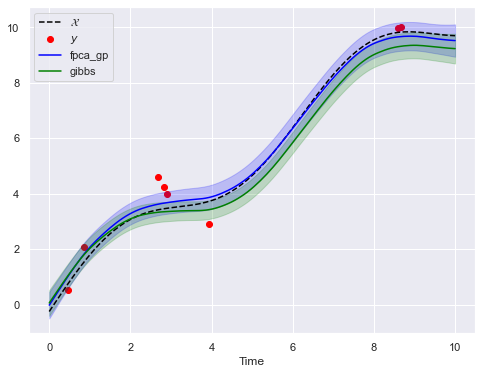
\includegraphics[width=\textwidth]{ex_val_A}
 	\caption[Example reconstruction using the CPACE model for Scenario A in our simulation study.]{An indicative example of the CPACE model performance on reconstruction of functional data where noisy observations have been made for Scenario A. The shaded regions represent our confidence interval of prediction and corresponds to two standard deviations from our mean predictions.}
 	\label{fig:val_ex_A}
 \end{figure}

Finally another advantage of the CPACE model is the ability to refine estimation of the noise variance and the component kernel variances, $\sigma_\varepsilon^2$ and $\lambda_k$  respectively.
While this, as shown in Table~\ref{tab:val_A}, may not gain much in reconstruction power this does indicate the CPACE framework`s ability to capture the true parameters of the model better. 
Figure~\ref{fig:noise_param_A} shows the distribution of the estimated noise variance over all our models. 
This distribution was estimated by smoothing the empirical distribution of the noise estimate from our $50$ replications of the simulation study.
Notice that the CPACE model`s tend to produce more consistent estimates than the standard PACE model.
This is because the CPACE framework allows for refinement of these estimates using the PACE estimate as an initial value through the Gaussian process likelihood of observed data.
Similar results are seen in the eigenvalue estimates (kernel variances).
Figure~\ref{fig:lambda_1_param_A} and Figure~\ref{fig:lambda_2_param_A} show this for the first and second eigenvalues respectively.
This is wanted and useful behaviour for modelling, as it provides assurance that the CPACE model can improve on the initial PACE estimates for both the noise parameter and variance parameters.
This should lead to improved understanding of the possible data generation procedure when using these models on real world data sets.

\begin{figure}
	\centering
	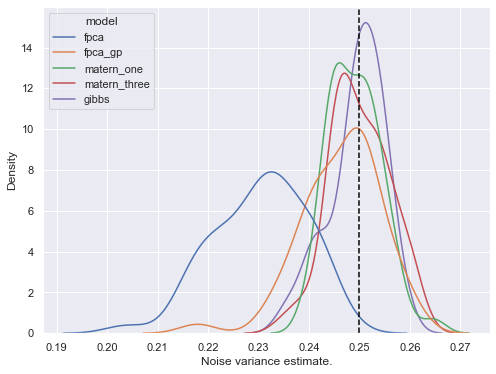
\includegraphics[width=\textwidth]{noise_param_A}
	\caption{Estimated noise variance distribution for each of our models over the 50 simulations for scenario A. The true noise variance is given by the vertical black line for indication.}
		\label{fig:noise_param_A}
\end{figure}

\begin{figure}
	\centering
	\begin{subfigure}[b]{0.45\textwidth}
 		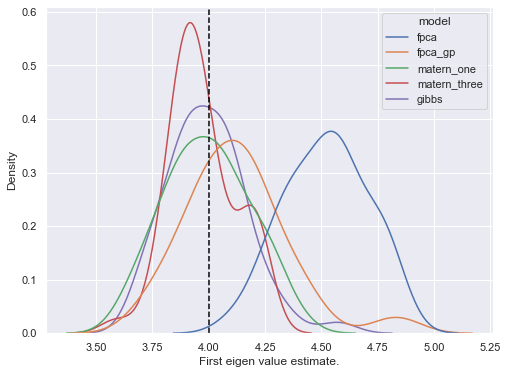
\includegraphics[width=\textwidth]{lambda_1_param_A}
 		\caption{Estimated first eigenvalue (first kernel variance) for each of our models over the 50 simulations for scenario A. The true parameter is given by the vertical black line for indication.}
 		\label{fig:lambda_1_param_A}
	\end{subfigure}
	\hfill
	\begin{subfigure}[b]{0.45\textwidth}
 		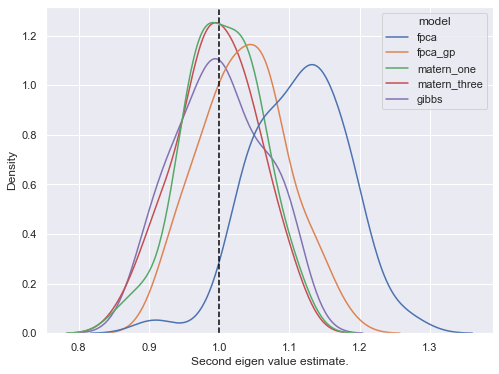
\includegraphics[width=\textwidth]{lambda_2_param_A}
 		\caption{Estimated second eigenvalue (second kernel variance) for each of our models over the 50 simulations for scenario A. The true parameter is given by the vertical black line for indication.}
 		\label{fig:lambda_2_param_A}
	\end{subfigure}
	\caption{Distributions of the estimated first and second eigenvalues for each model in Scenario A.}
	\label{fig:lambda_param_A}
\end{figure}

Next we consider the test results for this scenario study.
As described in Section~\ref{ssec:eval_metrics} the test results are metrics for the reconstruction ability on the test data set.
This is the set of locations in the domain $\mathcal{S}$ in which functional data are simulated but we assume we have no observations at these locations as all.
Table~\ref{tab:test_A} displays the $MSE$ and $MAE$ results for all our models.
Firstly; it is worth nothing that the metric results across all models for the test dataset are worse than that of the training and validation datasets, see Table~\ref{tab:train_A},~\ref{tab:val_A} respectively.
This is understandable, due to the nature of this scenario, since we are considering spatially independent functional data.
As expected both the \verb*|fpca| and \verb*|fpca_gp| model produce similar results which are the best possible under our simulation study models.
They are similar as both models will predict the mean function at unobserved locations, due to the structure of the White kernel upon which they depend.
It is expected that these models will produce the best in class results as they most closely represent the simulated data generation. 
Again, it is however worth noting that the other models have generalised well by estimation of their appropriate length scales.
This bodes well, as supports the use of these models in the case where the model may have small spatial structure and it is unknown as to whether to use a spatial model or not.
These simulation results suggest that you are not hindered by choosing a more complex kernel which may take into account spatial dependency; since the CPACE model will approximate spatial independence by adjusting the kernel hyper parameters appropriately.
However there are limitations.
The comparatively poor performance of the \verb*|gibbs| model may be because the complexity of this model has lead to non-convergence of the length scale models, leading to spurious spatial dependence.
This would then lead to less accurate forecast and giving higher test metrics.
We discuss the implementation we have used to minimise this in Chapter~\ref{cha:implementation}.
This issue wasn't present CPACE models using the Mat\'ern based kernels.

\begin{table}
	\caption[Simulation results for Scenario A on test data]{Simulation results for Scenario A on the model's ability to estimate the functional data at locations with no observation across the whole temporal domain. Bold indicates best in class.}
	\centering
	\label{tab:test_A}
	\begin{tabular}{lcc}
		\toprule
		\textbf{Model} & \textbf{MSE} & \textbf{MAE} \\
		\midrule
		\verb*|pace| & \textbf{5.0105 (0.1234)} & \textbf{5.5143 (0.0645)} \\
		\verb*|fpca_gp| & \textbf{5.0105 (0.1234)} & \textbf{5.5143 (0.0645)} \\
		\verb*|matern_one| & 5.3783	(0.2622) & 5.7094 (0.1298) \\
		\verb*|matern_three| & 5.5190 (0.4540) & 5.7824	(0.2262) \\
		\verb*|gibbs| & 6.6118 (0.4765) & 6.2981 (0.1987)\\
		\bottomrule
	\end{tabular}
\end{table}

\section{Scenario B - Stationary Functional Data \label{sec:sim_B}}
The next scenario we consider under our simulation study is the case of simulated data which exhibits spatial dependence.
We assume for scenario B that we have stationary dependence.
We induce this by considering that each component spatial covariance is given by the Mat\'ern One Half covariance model.
For both components we assume the length scale for the Mat\'ern One Half covariance is 2.
In essence, we are considering here a simple case of spatial dependence, as both components have the same spatial covariance structure.
Figure~\ref{fig:ex_spa_B} gives an example of what the full simulated data looks like over space.
This is for illustration only, to give the reader an idea of the scale of the spatial dependence induced.
This corresponds to only one realisation of the data generating procedure for scenario B at a particular time point.

\begin{figure}
	\centering
	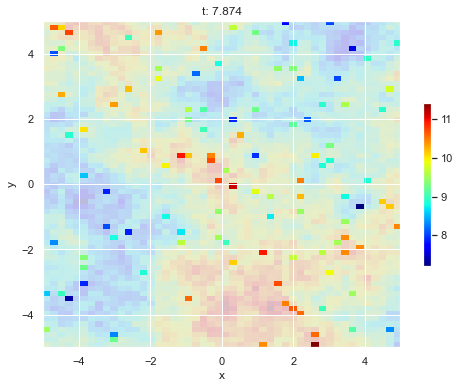
\includegraphics[width=\textwidth]{ex_spa_B}
	\caption{Example realisation of the spatial dependence under scenario B at a particular time point in domain $\mathcal{T}$. Here we show the full unobserved data across $\mathcal{S}$ with observed data being given by the less transparent pixels in the image.}
	\label{fig:ex_spa_B}
\end{figure}

Again we compare the same models as in Scenario A, see Section~\ref{sec:sim_A} for a full description.
Table~\ref{tab:train_B} reports the metric results for these models on Scenario B observed data.
As expected our Mat\'ern One Half model performs best on the training data.
Again, this is most probably because it closely resembles the data generating procedure for this scenario.
It is also important to note the significant improvement any spatial dependence in the model kernel makes for reconstruction on the training data.
Both the Mat\'ern One Half and Mat\'ern Three Halves models shows considerable improvements, but so does the Gibbs model although improvements are noticeable smaller.


\begin{table}
	\caption[Simulation results for Scenario B on observed data]{Simulation results for Scenario B for the model`s ability to estimate the functional data at points of observation. Bold indicates best in class.}
	\centering
	\label{tab:train_B}
	\begin{tabular}{lcc}
		\toprule
		\textbf{Model} & \textbf{MSE} & \textbf{MAE} \\
		\midrule
		\verb*|pace| & 0.0483 (0.0016) & 0.1738	(0.0029) \\
		\verb*|fpca_gp| & 0.0482 (0.0016) & 0.1736 (0.0029) \\
		\verb*|matern_one| & \textbf{0.0275	(0.0013)} & \textbf{0.1310	(0.0030)} \\
		\verb*|matern_three| & 0.0352 (0.0019) & 0.1477	(0.0040) \\
		\verb*|gibbs| & 0.0425 (0.0038) & 0.1613 (0.0071)\\
		\bottomrule
	\end{tabular}
\end{table}

We note as in Scenario A we have refined estimates for the error variance and eigenvalues (kernel variances) than from the PACE model under the CPACE framework. 
For Scenario B these estimates are displayed in Figures~\ref{fig:noise_param_B},~\ref{fig:lambda_1_param_B}, and~\ref{fig:lambda_2_param_B} respectively. 
We see that the noise estimate is more precise for the CPACE models compared to the PACE model.
However for the eigenvalue estimate we see the PACE model actually delivers more consistent results.
It is important to note that under spatial dependence it is possible for these to be biased away from the true values due to the correlation induced among functional observations.

\begin{figure}
	\centering
	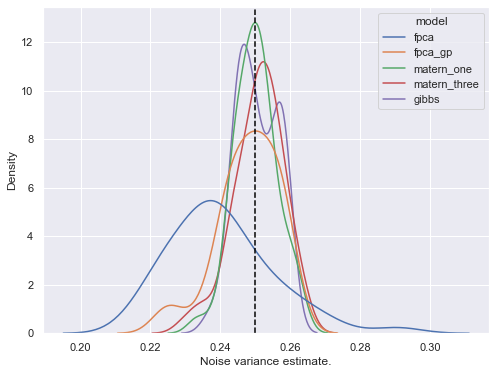
\includegraphics[width=\textwidth]{noise_param_B}
	\caption{Estimated noise variance distribution for each of our models over the 50 simulations for Scenario B. The true noise variance is given by the vertical black line for indication.}
	\label{fig:noise_param_B}
\end{figure}

\begin{figure}
	\centering
	\begin{subfigure}[b]{0.45\textwidth}
		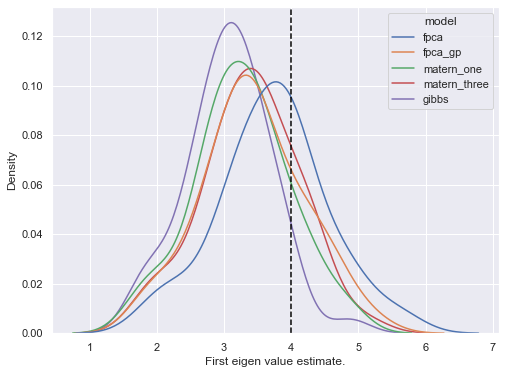
\includegraphics[width=\textwidth]{lambda_1_param_B}
		\caption{Estimated first eigenvalue (first kernel variance) for each of our models over the 50 simulations for Scenario B. The true parameter is given by the vertical black line for indication.}
		\label{fig:lambda_1_param_B}
	\end{subfigure}
	\hfill
	\begin{subfigure}[b]{0.45\textwidth}
		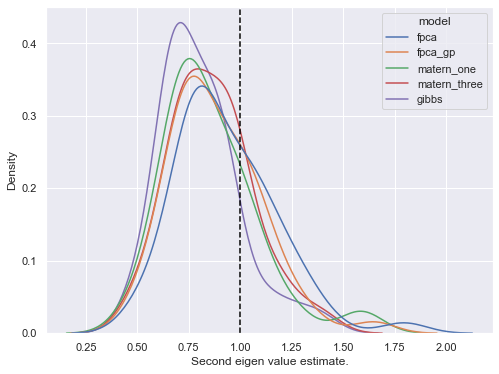
\includegraphics[width=\textwidth]{lambda_2_param_B}
		\caption{Estimated second eigenvalue (second kernel variance) for each of our models over the 50 simulations for Scenario B. The true parameter is given by the vertical black line for indication.}
		\label{fig:lambda_2_param_B}
	\end{subfigure}
	\caption{Distributions of the estimated first and second eigenvalues for each model in Scenario B.}
	\label{fig:lambda_param_B}
\end{figure}

In Scenario B we also can compare the length scale estimate from the Mat\'ern based models to that of the scenario for each component.
As we can see in Figure~\ref{fig:rho_1_param_B} and Figure~\ref{fig:rho_2_param_B} the Mat\'ern One Half model manages to capture the true value in its distribution for each component, although it resides in the tail of the distribution.
This may indicate that it hasn't quite captured the data generating procedure entirely, however coupled with the underestimate of the kernel variance, an underestimate of the kernel length scale does make sense.
The Mat\'ern Three Halves model fails to capture the true length scale parameter in its model, but again as this model is inherently smoother over larger distances this makes sense that the length scale would be smaller when estimated on this scenario to account for this.
\begin{figure}
	\centering
	\begin{subfigure}[b]{0.45\textwidth}
		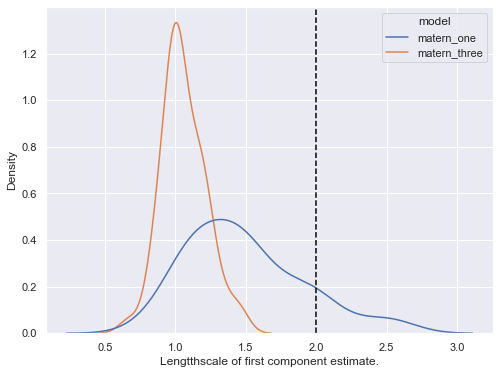
\includegraphics[width=\textwidth]{rho_1_param_B}
		\caption{Estimated first kernel length scale parameter for the Mat\'ern models over the 50 simulations for Scenario B. The true parameter is given by the vertical black line for indication.}
		\label{fig:rho_1_param_B}
	\end{subfigure}
	\hfill
	\begin{subfigure}[b]{0.45\textwidth}
		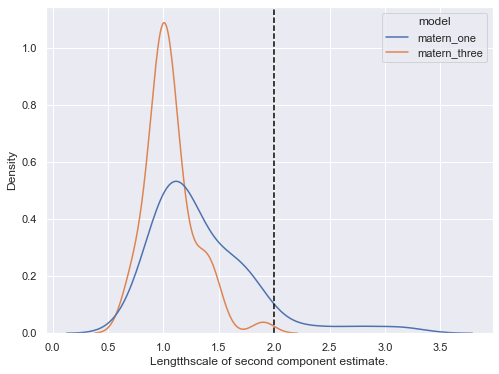
\includegraphics[width=\textwidth]{rho_2_param_B}
		\caption{Estimated second kernel length scale parameter for the Mat\'ern models over the 50 simulations for Scenario B. The true parameter is given by the vertical black line for indication.}
		\label{fig:rho_2_param_B}
	\end{subfigure}
	\caption{Distributions of the estimated first and second length scale parameters for each model in Scenario B.}
	\label{fig:rho_param_B}
\end{figure}

We now consider the test metrics for these models.
Table~\ref{tab:test_B} showcases these results.
As expected these results highlight that the Mat\'ern One Half model succeeds in being the most accurate of the models for reconstructing completely unobserved functional data.
As can also be seen the Mat\'ern Three Halves model comes surprisingly close to recreating the simulated data.
This is again showcasing the ability of the CPACE framework to tailor the hyper parameters of the chosen kernel to suitably capture the data.
In this case we have seen, from Figure~\ref{fig:rho_1_param_B}, that this corresponds to estimating the shorter length scale hyper parameter to compensate for the smoother kernel function.
However, it doesn't quite compensate for having the correct kernel for the data generating procedure, which is why the Mat\'ern One Half kernel obtains the best metrics.
As the standard deviation of the Mat\'ern One Half and Mat\'ern Three Halves metrics indicate that they may well in fact be equally as powerful, we use the distribution of metric results to highlight the Mat\'ern One Half model to be best in class.
Figure~\ref{fig:test_comp_B} highlights the distribution of metrics over the full 50 simulations between these two models.
In this type of plot the smoothed empirical distribution of the metric is represented by the shape with the mean, interquartile range, and range being given by the bar inside the shape. 
We can see a slightly more positive skew for the distribution of both $MAE$ and $MSE$ for the Mat\'ern One Half model, again indicating that this model is more consistent in reconstruction that the Mat\'ern Three Halves model.
Hence we conclude that the Mat\'ern One Half model constitutes our best in class on the test data set for scenario B. 

We can see quite clearly that the PACE and CPACE framework of the PACE model are not flexible enough to help on unobserved functional data, from Table~\ref{tab:test_B}.
As due to their White kernel they only propose the mean for all unobserved data.
While this was advantageous in Scenario A, under spatial correlation between functional data this becomes a hindrance. 

\begin{table}
	\caption[Simulation results for Scenario B on test data]{Simulation results for Scenario B for the model`s ability to estimate the functional data at locations with no observation across the whole temporal domain. Bold indicates best in class.}
	\centering
	\label{tab:test_B}
	\begin{tabular}{lcc}
		\toprule
		\textbf{Model} & \textbf{MSE} & \textbf{MAE} \\
		\midrule
		\verb*|pace| & 4.1851 (0.7638) & 5.0613	(0.4810) \\
		\verb*|fpca_gp| & 4.1851 (0.7638) & 5.0613 (0.4810) \\
		\verb*|matern_one| & \textbf{0.5848	(0.0215)} & \textbf{1.8926	(0.0333)} \\
		\verb*|matern_three| & 0.5967 (0.0212) & 1.9100	(0.0323) \\
		\verb*|gibbs| & 0.7413 (0.0505) & 2.1187 (0.0666)\\
		\bottomrule
	\end{tabular}
\end{table}

\begin{figure}
	\centering
	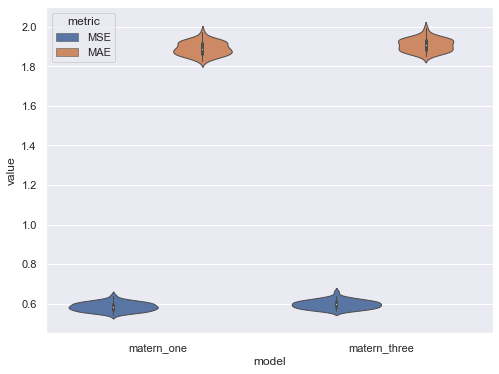
\includegraphics[width=\textwidth]{comp_test_B}
	\caption[Distribution of the $MSE$ and $MAE$ metrics over the $50$ simulations for the test data set of scenario B.]{Distribution of the $MSE$ and $MAE$ metrics over the $50$ simulations for the test data set of scenario B. Here the shape represents the smoothed empirical distribution of the metric while the summary statistics of the mean, interquartile range, and range are given from the bars inside the shape.}
	\label{fig:test_comp_B}
\end{figure}

Finally, to highlight the abilities of the CPACE models, we display an example prediction of a test data location in Figure~\ref{fig:test_ex_B}.
Here we clearly see the reconstruction ability of the CPACE framework and the higher confidence in reconstruction that the CPACE framework can bring.
This is applicable to both the Mat\'ern One Half and Mat\'ern Three Halves models.
We can also see the advantage of the Mat\'ern One Half model, as although the confidence band is much narrower than the PACE model under the CPACE framework it isn't as narrow as the Mat\'ern Three Halves model.
This is advantageous as can be seen in Figure~\ref{fig:test_ex_B}.
The actual functional data sometimes falls outside the Mat\'ern Three Halves confidence band but still resides in the Mat\'ern One Half model.
This can be seen as an indicative example only, but may suggest the Mat\'ern Three Halves model may be over confident in its predictions on the test data, which stems from the fact that the kernel itself is too smooth for the data generating procedure. 
The Mat\'ern One Half model has no such issues.

\begin{figure}
	\centering
	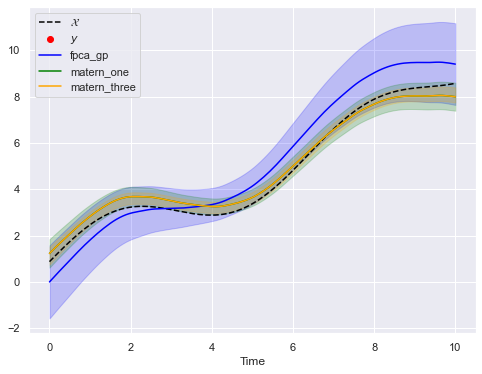
\includegraphics[width=\textwidth]{test_ex_B}
	\caption[An indicative example of the CPACE model performance on reconstruction of functional data for Scenario B.]{An indicative example of the CPACE model performance on reconstruction of functional data for Scenario B. Example is taken from a test data point, so no observations were observed at this spatial location. The confidence band correspond to a 95\% simultaneous confidence interval for the predicted location.}
	\label{fig:test_ex_B}
\end{figure}

From the above we can see an distinct advantage for using the CPACE framework when there is indeed simple spatial dependence, however this is as expected, and has been discussed in work by \citeauthor{liu_functional_2017}, \citep{liu_functional_2017}.
In the following sections we consider the more challenging case when the spatial dependence is more complex.

\section{Scenario C - Complex Stationary Functional Data \label{sec:sim_C}}

In this scenario we consider modelling simulations which are generated with a more challenging spatial dependence.
In particular, in this scenario we generate functional data as mentioned in Section~\ref{ssec:dgp_sim} but this time we place different spatial kernels on each component of the model.
We use the Mat\'ern Three Halves kernel for both components but choose a length scale of $3$ for the first component and a length scale parameter of $1.5$ for the second component.
In essence, we are now considering the case where there are two distinct covariance structures between the spatial components of the models.
Previous scenarios had the same spatial covariance for both components.
This scenario is designed as a test for the CPACE framework, to see if it can accommodate this added complexity.
Figure~\ref{fig:sim_example_C} highlights an example of a realisation of each of these covariance components. 
This is intended to highlight the spatial dependency present in such a simulation from each of the components.

\begin{figure}
	\centering
	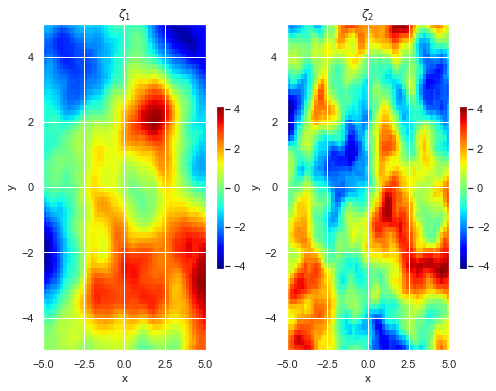
\includegraphics[width=\textwidth]{sim_ex_zeta_C}
	\caption{An indicative example of a realisation from the component spatial kernels in scenario C.}
	\label{fig:sim_example_C}
\end{figure}

As in previous scenarios we first consider the resultant metrics from the training data.
The results are displayed in Table~\ref{tab:train_C}.
As with the other scenarios, all models provided reasonable reconstruction on observed data.
This includes the PACE framework.
However, we can see a clear improvement in the metrics for the CPACE framework on the training data.
This is indicative that the CPACE models, through using the learned spatial dependence, can use this extra information to gain an advantage in reconstruction the fuunctional data from points of observation.
Again, as expected the model which performs best is the \verb*|matern_three| model as it closely relates to the data generating process. 
We can see this from Figure~\ref{fig:rho_1_param_C} and Figure~\ref{fig:rho_2_param_C}. 
These highlight that the \verb*|matern_three| model captures, although not perfectly, the true length scale parameters of the data generating process.
Similarly, the \verb*|matern_one| also captures the true length scale parameter, albeit with less certainty.
This is another indication that the CPACE frame for learning hyper parameters of the spatial kernels works well. 
This will be discussed further in Chapter~\ref{cha:implementation}.

\begin{table}
	\caption[Simulation results for Scenario C on observed data]{Simulation results for Scenario C for the models ability to estimate the functional data at points of observation. Bold indicates best in class.}
	\centering
	\label{tab:train_C}
	\begin{tabular}{lcc}
		\toprule
		\textbf{Model} & \textbf{MSE} & \textbf{MAE} \\
		\midrule
		\verb*|pace| & 0.0479 (0.0021)& 0.1733	(0.0038)\\
		\verb*|fpca_gp| & 0.0479 (0.0022) & 0.1731	(0.0039) \\
		\verb*|matern_one| & 0.0132	(0.0013) & 0.0909 (0.0044) \\
		\verb*|matern_three| & \textbf{0.0085 (0.0009)} & \textbf{ 0.0730	(0.0038)} \\
		\verb*|gibbs| & 0.0094	(0.0009) & 0.0767 (0.0036)\\
		\bottomrule
	\end{tabular}
\end{table}

\begin{figure}
	\centering
	\begin{subfigure}[b]{0.45\textwidth}
		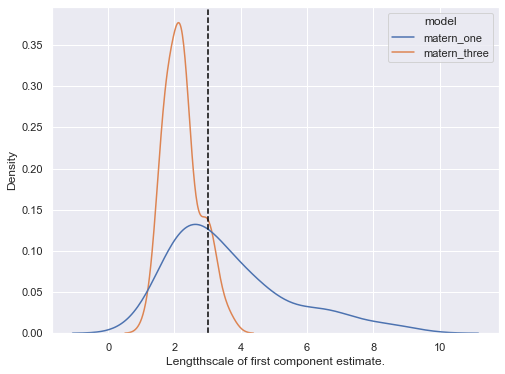
\includegraphics[width=\textwidth]{rho_1_param_C}
		\caption{Estimated first kernel length scale parameter for the Mat\'ern models over the 50 simulations for scenario C. The true parameter is given by the vertical black line for indication.}
		\label{fig:rho_1_param_C}
	\end{subfigure}
	\hfill
	\begin{subfigure}[b]{0.45\textwidth}
		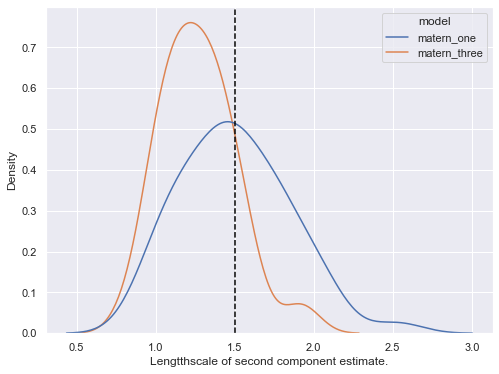
\includegraphics[width=\textwidth]{rho_2_param_C}
		\caption{Estimated second kernel length scale parameter for the Mat\'ern models over the 50 simulations for scenario C. The true parameter is given by the vertical black line for indication.}
		\label{fig:rho_2_param_C}
	\end{subfigure}
	\caption{Distributions of the estimated first and second length scale parameters for each model in Scenario C.}
	\label{fig:rho_param_C}
\end{figure}

We can see an indicative example for reconstruction of the data using the best in class \verb*|matern_three| model and the \verb*|fpca_gp| model in Figure~\ref{fig:sim_val_recon_C}.
This highlights the difference, not only in accuracy in reconstruction, but also the improved confidence of estimation of the best in class model.
We note that in areas far away (in the temporal domain) from observation, the \verb*|fpca_gp| model tends to revert to the mean function, and its confidence interval expands.
On the other hand the Mat\'ern Three Halves model can use information about observations from other spatial locations to improve its estimation for these areas.

\begin{figure}
	\centering
	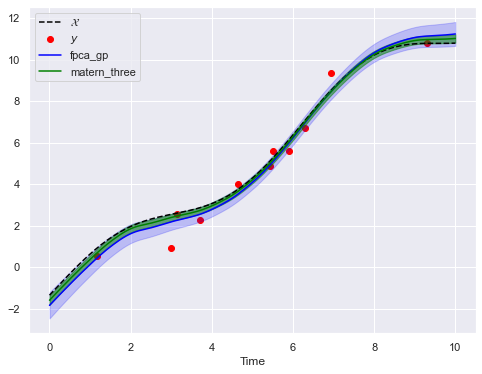
\includegraphics[width=\textwidth]{sim_val_recon_C}
	\caption[An indicative example of model reconstructions  for Scenario C for functional data with observed values.]{An indicative example of model reconstructions  for Scenario C for functional data with observed values. The shaded region is the prediction confidence band and corresponds to a 95\% simultaneous confidence interval.}
	\label{fig:sim_val_recon_C}
\end{figure}

Next we consider the models comparative ability for reconstruction of completely unobserved functional data.
Table~\ref{tab:test_C} displays our models results on the test data set for Scenario C.
Here, we see similar results to the training metrics, where the CPACE framework out performs the PACE models.
It is interesting to note here that the \verb*|gibbs| model outperforms the \verb*|matern_one|, although very slightly.
It again suggest the CPACE framework is capable of flexibly estimating kernel hyper parameters, even when the parameter space is relatively large as in the case of the Gibbs kernel.
We note that we have highlighted the \verb*|matern_three| as best in class due to slightly larger positive skew in distribution of metrics over the test data set versus the \verb*|gibbs| model. 
This is evidenced in Figure~\ref{fig:test_met_C}.
In Figure~\ref{fig:test_met_C} we compare only the \verb*|fpca_gp| and \verb*|matern_three|, this is to make it easier to see the comparative difference between best in class and the standard PACE model.
We note that the \verb*|matern_one| and \verb*|gibbs| models produce similar reconstructions to that of \verb*|matern_three|.

\begin{table}
	\caption[Simulation results for Scenario C on test data]{Simulation results for the models ability to estimate the functional data at locations with no observations across the whole temporal domain. Bold indicates best in class.}
	\centering
	\label{tab:test_C}
	\begin{tabular}{lcc}
		\toprule
		\textbf{Model} & \textbf{MSE} & \textbf{MAE} \\
		\midrule
		\verb*|pace| & 3.3175 (0.9034) & 4.5480	(0.6234) \\
		\verb*|fpca_gp| & 3.3175 (0.9034) & 4.5480	(0.6234)  \\
		\verb*|matern_one| & 0.1109	(0.0112) & 0.8343 (0.0410) \\
		\verb*|matern_three| & \textbf{0.0957 (0.0104)} & \textbf{0.7745 (0.0412)} \\
		\verb*|gibbs| & 0.1053 (0.0106) & 0.8117 (0.0400)\\
		\bottomrule
	\end{tabular}
\end{table}

\begin{figure}
	\centering
	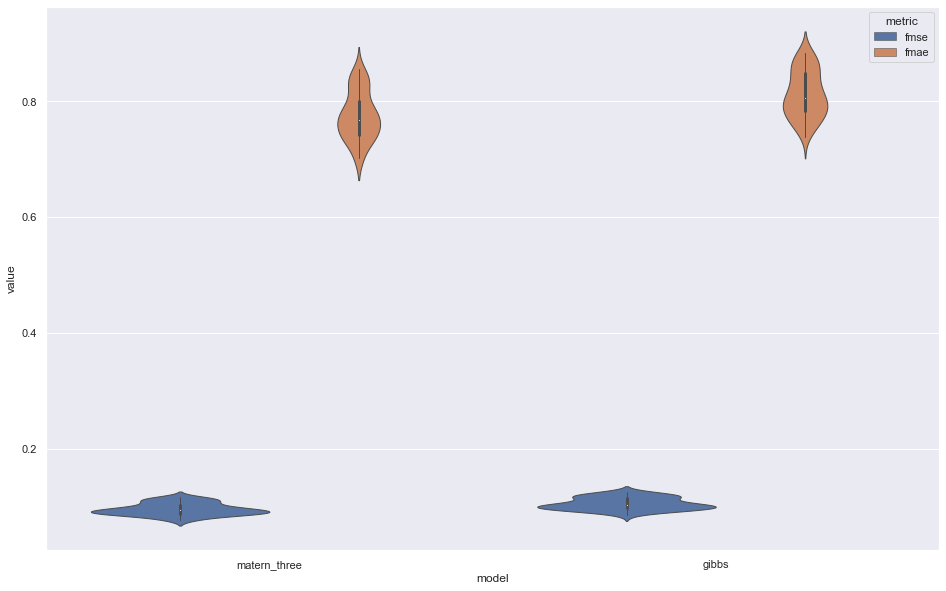
\includegraphics[width=\textwidth]{test_met_C}
	\caption[Test metric distribution for Scenario C over $50$ simulations for the Mat\'ern Three Halves and Gibbs model.]{Test metric distribution for Scenario C over $50$ simulations for the Mat\'ern Three Halves and Gibbs model.  Here the shape represents the smoothed empirical distribution of the metric while the summary statistics of the mean, interquartile range, and range are given from the bars inside the shape.}
	\label{fig:test_met_C}
\end{figure}

Finally we give an indicative example of reconstruction using the best in class model and the \verb*|fpca_gp| model to highlight the improvement in reconstruction. 
This is given in Figure~\ref{fig:sim_test_recon_C}. 
We can clearly see the ability of the CPACE framework here to utilise the spatial dependency between observations, not only in reconstruction accuracy but in confidence of prediction.
As can be seen, the CPACE framework has allowed for models which can handle quite complex spatial models. 
This has a real advantage in terms of both prediction accuracy and confidence in prediction on both unobserved locations and locations with observation points. 

\begin{figure}
	\centering
	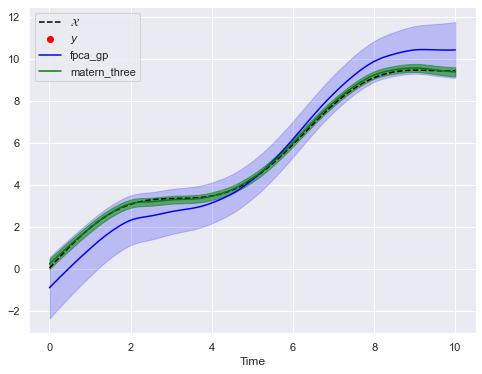
\includegraphics[width=\textwidth]{sim_test_recon_C}
	\caption[An indicative example of model reconstructions for Scenario C for functional data with no observations.]{An indicative example of model reconstructions for Scenario C for functional data with no observations. The shaded region is the prediction confidence band and corresponds to a 95\% simultaneous confidence interval.}
	\label{fig:sim_test_recon_C}
\end{figure}

In the final scenario we consider one further step of complexity.
That is we examine the CPACE frameworks ability to handle data which is simulated with a non-stationary spatial dependency. 

\section{Scenario D - Non-Stationary Functional Data \label{sec:sim_D}}
In the final scenario of the simulation study, we consider the case of data being generated which has non-stationary spatial dependency.
We do so by simulating data for this scenario, following the data generation procedure given in Section~\ref{ssec:dgp_sim}, and use a Gibbs kernel for each component.
We choose our length scale models for the scenario so that we create a non stationary spatial dependence.
In particular, we choose a two component Gibbs kernel to simulate from. 
The length scale model for each components is given by:

\begin{eqnarray}
	l_1(s) &=& \frac{1}{1 + \exp(-s)} \nonumber \\
	l_2(s) &=& \frac{1}{1 +  \exp(s)} \nonumber \\
\end{eqnarray}
where, as mentioned before, the Gibbs kernel is extended to multiple dimensions by applying the Gibbs kernel over each separate dimension of the domain $\mathcal{S}$. 
An indicative example of the scores that are generated from these kernels is given in Figure~\ref{fig:sim_ex_zeta_D}. 
As can be seen, the realised scores for each kernel have a similar structure, but are clearly non-stationary, with the corners of the domain having least structure while the middle of the domain has fairly strong structure.
A corresponding example realisation from this scenario is displayed in Figure~\ref{fig:sim_example_D}.
This highlights how the non-stationary score processes manifest in the scenario simulations.

\begin{figure}
	\centering
	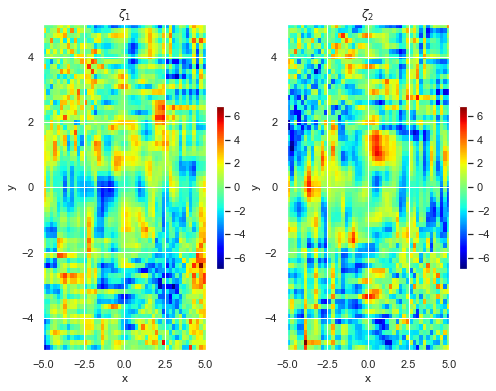
\includegraphics[width=\textwidth]{sim_ex_zeta_D}
	\caption{Realisation from score processes corresponding to scenario D.}
	\label{fig:sim_ex_zeta_D}
\end{figure}

\begin{figure}
	\centering
	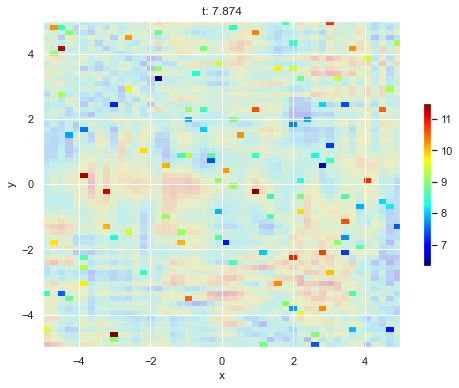
\includegraphics[width=\textwidth]{sim_example_D}
	\caption[Spatial view of a particular time point in $\mathcal{T}$ from a realisation from scenario D.]{Spatial view of a particular time point in $\mathcal{T}$ from a realisation from scenario D. This realisation corresponds to the example score realisation in Figure~\ref{fig:sim_ex_zeta_D}. The darker pixels correspond to the noisy observations, with the lighter pixels representing unobserved locations at this time point.}
	\label{fig:sim_example_D}
\end{figure}

For the study itself, we first present the training metrics of our various prospective models. 
This is displayed in Table~\ref{tab:train_D}.
As we can see the best in class model on the training metric is the Mat\'ern One Half model. 
However, all the models perform comparatively as well as each other.
The Mat\'ern One Half model is chosen as best in class based on its overall performance.
If we look at the distribution of the metrics over the $50$ simulations, Figure~\ref{fig:train_D_dist}, we see that it is on average the best performer. 
However we can see the Gibbs model  does have the optimal performance, but also the largest range in performance over the simulations of both metrics.
We can see that the PACE and White kernel models also perform well on the training metrics.
We account for this as although the simulations has spatial dependency, some of this spatial dependency is quite weak.
For example at the corners of the domain $\mathcal{S}$ and so a reasonable approximation to the data generating procedure at these locations would be the White kernel CPACE models.


\begin{table}[b]
	\caption[Simulation results for Scenario D on observed data]{Simulation results for the models ability to estimate the functional data at points of observation. Bold indicates best in class.}
	\centering
	\label{tab:train_D}
	\begin{tabular}{lcc}
		\toprule
		\textbf{Model} & \textbf{MSE} & \textbf{MAE} \\
		\midrule
		\verb*|pace| & 0.0503 (0.0017)& 0.1772 (0.0030)\\
		\verb*|fpca_gp| & 0.0501 (0.0017) & 0.1768	(0.0029) \\
		\verb*|matern_one| & \textbf{0.0447	(0.0015)} & \textbf{0.1667 (0.0027)} \\
		\verb*|matern_three| & 0.0532 (0.0052)& 0.1802 (0.0077) \\
		\verb*|gibbs| & 0.0542 (0.0079) & 0.1785 (0.0109)\\
		\bottomrule
	\end{tabular}
\end{table}

\begin{figure}
	\centering
	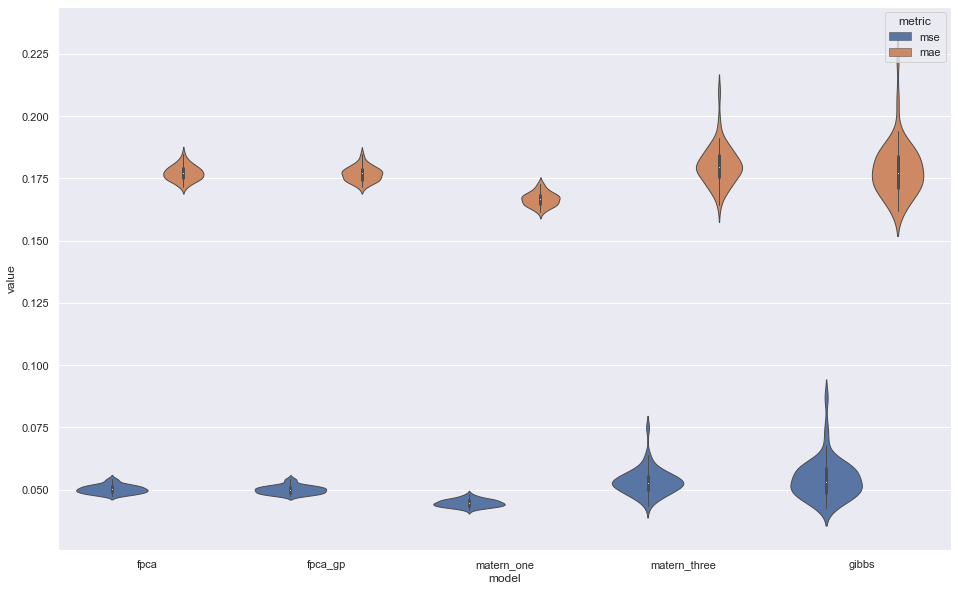
\includegraphics[width=\textwidth]{train_D_dist}
	\caption{Distribution of metrics, $MAE$ and $MSE$ over the training data for each simulation in Scenario D.}
	\label{fig:train_D_dist}
\end{figure}

We now consider the resulting metrics on the test data set for Scenario D.
Table~\ref{tab:test_D} displays these.
Here we can see that on the test data, the Gibbs model becomes the best in class.
We can see that the models with spatial dependency have an advantage over those which do not, which is as expected.
The Gibbs model seems to have captured that added complexity in this scenario, by allowing for a non-stationary structure. 
This has given the model the edge in the ability to reconstruct unobserved data.
However, it is worth noting that the Gibbs model has the largest variance in metric results of the models with a non-White kernel.
This probably indicates that there is a possibility that using the more complex kernel in the CPACE framework means the estimation of hyper parameters may not always converge at the optimum values.
This is a common situation for models where the parameter space is large and optimising for the optimal parameters may sometimes land in a local optimum rather than a global optimum. 
This issue, and how we attempted to minimise this issue, is discussed in Chapter~\ref{cha:implementation}.
Finally, for illustration, we provide an example reconstruction of an unobserved location for the \verb*|fpca_gp| and \verb*|gibbs| models in Figure~\ref{fig:sim_test_recon_D}.
Here we can clearly see the improvement in prediction from using the CPACE framework, both for mean prediction and confidence of prediction.

\begin{figure}
	\centering
	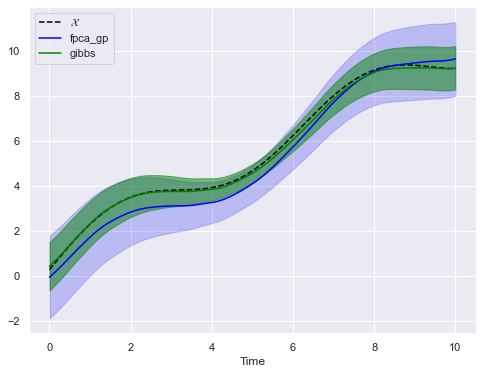
\includegraphics[width=\textwidth]{sim_test_recon_D}
	\caption[An indicative example of model reconstructions for Scenario D for functional data with no observations.]{An indicative example of model reconstructions for Scenario D for functional data with no observations. The shaded region is the prediction confidence band and corresponds to a 95\% simultaneous confidence interval.}
	\label{fig:sim_test_recon_D}
\end{figure}

\begin{table}[b]
	\caption[Simulation results for Scenario D on test data]{Simulation results for the models ability to estimate the functional data at points of observation. Bold indicates best in class.}
	\centering
	\label{tab:test_D}
	\begin{tabular}{lcc}
		\toprule
		\textbf{Model} & \textbf{MSE} & \textbf{MAE} \\
		\midrule
		\verb*|pace| & 4.9249 (0.4543)& 5.4494 (0.2338)\\
		\verb*|fpca_gp| & 4.9249 (0.4543)& 5.4494 (0.2338)\\
		\verb*|matern_one| & 2.4335	(0.1310) & 3.7206 (0.0901) \\
		\verb*|matern_three| & 2.6123 (0.1446)& 3.8147 (0.0952) \\
		\verb*|gibbs| & \textbf{2.0135 (0.2170)} & \textbf{3.3181 (0.1806)}\\
		\bottomrule
	\end{tabular}
\end{table}

\section{Summary\label{sec:sim_summ}}
In this chapter we have considered a simulation study to assess the ability of the CPACE model in various conditions.
Our primary aim was to compare the CPACE model, which introduces explicitly modelling spatial dependence between functional observations, with the standard PACE modelling.
We consider four different scenarios with various levels of spatial dependence, to assess how the CPACE framework behaves.
In these scenarios we considered using 4 different models under the CPACE framework, each utilising a different assumed form of the score processes.
We have seen, from Scenario A results, that regardless of the assumed form of the score process, the CPACE framework can effectively mimic the PACE framework.
This is achieved by estimating hyper parameters for the score processes that cause these to mimic the White kernel. 
Further, we have seen through Scenarios B and C that the CPACE model can accommodate stationary spatial dependence between functional observations.
Here we saw that choosing the assumed score process as close to the data generating procedure is obviously the preferred choice, but using a score process which is flexible enough to accommodate  stationary spatial dependency will give similar results.
Finally, we tested the CPACE model on data which has a complex non-stationary spatial dependency between functional observations.
Here, on training data the assumed score process chosen seemed not to mater too much. 
However, when looking at metrics on the test data we saw clearly that the models which assumed only a stationary score process were outperformed by the Gibbs model.
This underlines a common theme. That is, assuming a slightly more complex form of the score process under the CPACE framework tends to work better for test data reconstruction.
This is because the CPACE framework allows nicely for tuning of hyper parameters so that complex forms can estimate simpler forms, however the reverse is not true. 
For example, one cannot choose hyper parameters of the Mat\'ern kernel such that it becomes non-stationary.
Whereas we can make the Gibbs kernel stationary by assuming the length scale model is constant over the spatial domain. 

We have highlighted the pros and cons of the CPACE model, and contrasted this with the ability of the PACE model on simulated data.
We proceed to discuss the CPACE model on our real world data, the CESM-LE dataset (see Chapter~\ref{cha:data} for an in-depth description), in Chapter~\ref{cha:real_application}.
We discuss the implementation of the CPACE model, which mainly revolves around the hyper parameter estimation of the assumed scores processes in Chapter~\ref{cha:implementation}.



